\chapter{Аналитический раздел}

\section{Анализ существующих решений}

Для сравнения существующих решений были выделены следующие критерии:
\begin{itemize}
	\item[---] K1: Авторизация (поддерживается/не поддерживается);
	\item[---] K2: История (поддерживается/не поддерживается);
	\item[---] K3: Цена (платно/бесплатно);
	\item[---] K4: Управление транспортной моделью в реальном времени (поддерживается/не поддерживается);
\end{itemize}

Результаты сравнения существующих решений приведены в таблице~\ref{tbl:cmp}.
\begin{table}[h]
	\begin{center}
		\caption{\label{tbl:cmp} Сравнение решений}
		\begin{tabular}{|c|c|c|c|c|c|}
			\hline
			Решение & K1 & K2 & K3 & K4 \\
			\hline
			Яндекс.Метро & -- & -- & + & -- \\
			\hline
			Google maps & + & + & + & -- \\
			\hline
			Moovit & + & + & +/-- & -- \\
			\hline
			Transit & + & + & + & -- \\
			\hline
			Metro & -- & -- & +/-- & -- \\
			\hline
			Разрабатываемое решение & + & + & + & + \\
			\hline
		\end{tabular}
	\end{center}
\end{table}

Проведенный сравнительный анализ подтверждает, что разрабатываемая система обладает конкурентным преимуществом за счет поддержки динамического редактирования транспортной модели.

\section{Формализация задачи}

В рамках курсовой работы требуется спроектировать и разработать базу данных для хранения информации о схемах метро -- структурах связанных сущностей таких как: ветки, станции, переезды и переходы. А также о пользователях и маршрутах, которые могут быть сохрянены в истории конкретного пользователя. Необходимо разработать серверное приложение взаимодействующее с базой данных, реализующее поиск маршрутов и позволяющее изменять параметры схемы метро для пользователей с определенными правами.

На рисунке~\ref{chart:usecase} представлена диаграмма прецедентов для разных ролей пользователей.

\begin{figure}[h]
    \centering
    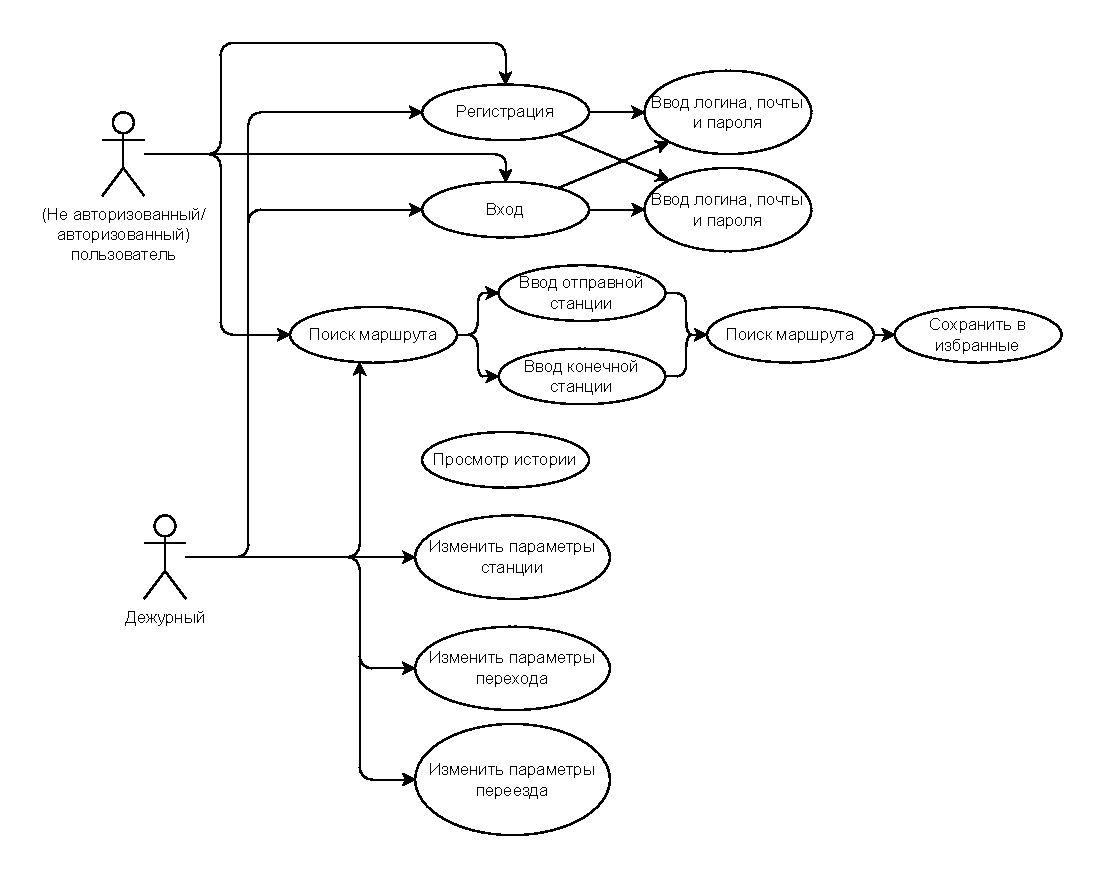
\includegraphics[width=\textwidth]{inc/img/use-case.pdf}
    \caption{Диаграмма прецедентов разных ролей}
    \label{chart:usecase}
\end{figure}

\FloatBarrier

На рисунке~\ref{chart:BPMN} представлена диаграмма ключевых бизнес-процессов.

\begin{figure}[h]
    \centering
    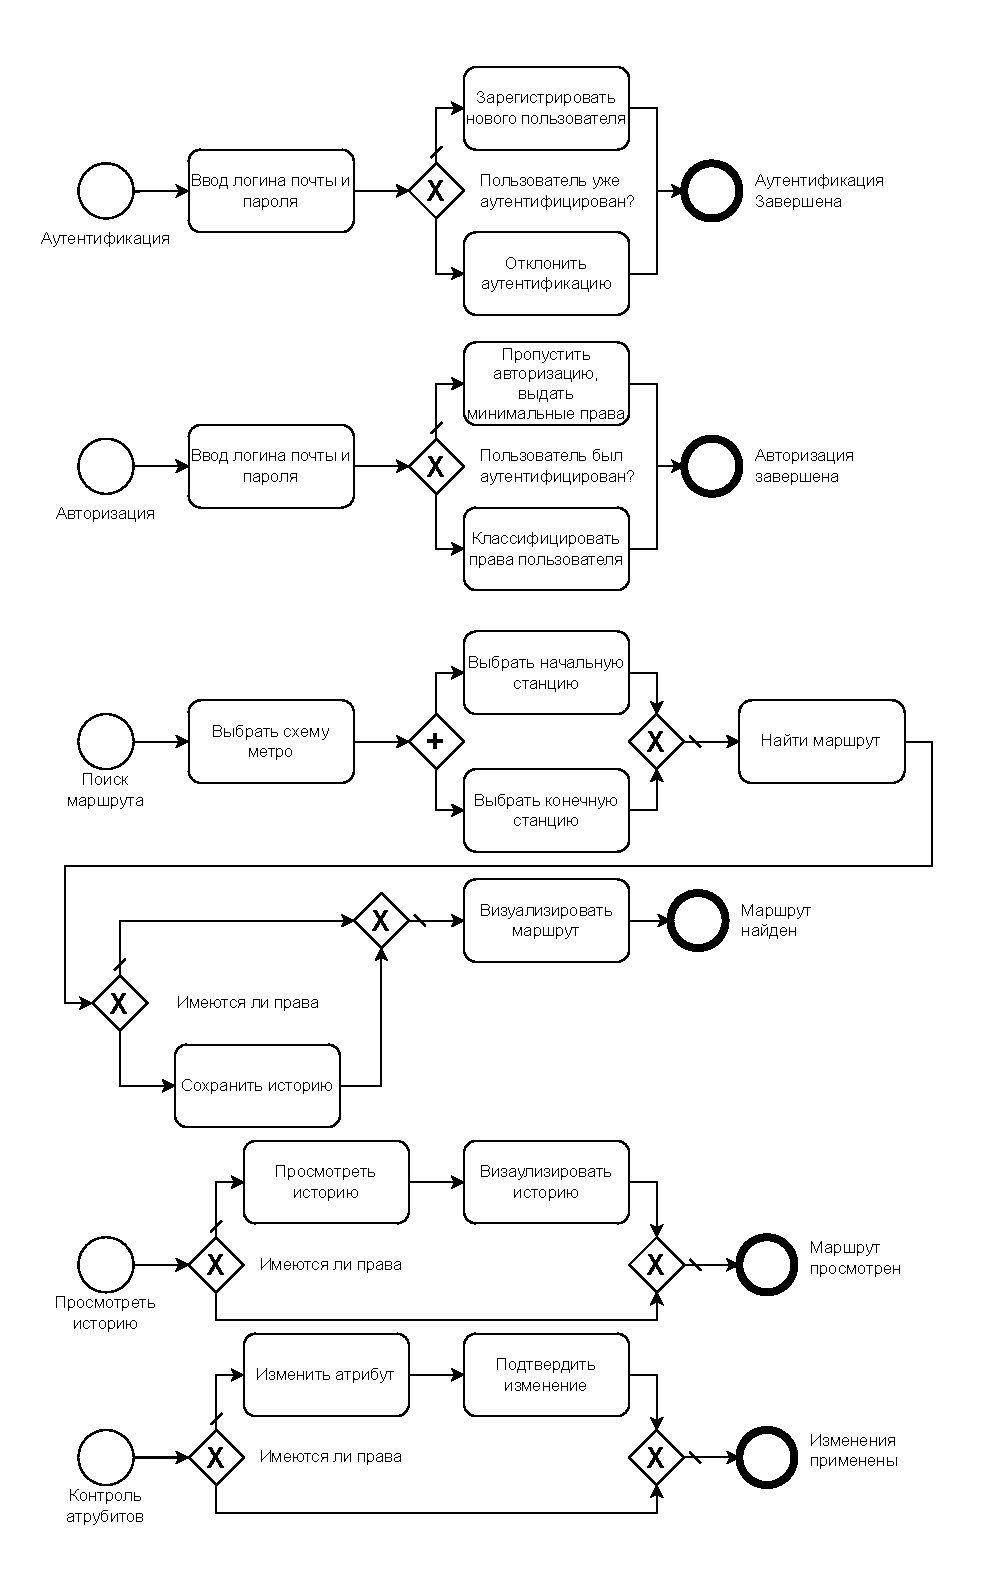
\includegraphics[width=0.8\textwidth]{inc/img/BPMN.pdf}
    \caption{Диаграмма прецедентов разных ролей}
    \label{chart:BPMN}
\end{figure}

\FloatBarrier

\section{Формализация данных}

База данных должна хранить информацию о:
\begin{itemize}
	\item[---] пользователях;
	\item[---] cхемах метро;
	\item[---] ветках;
	\item[---] станциях;
	\item[---] переездах;
	\item[---] переходах;
	\item[---] маршрутах.
\end{itemize}

В таблице \ref{tbl:crt} указаны хранимые сущности и их характеристики.

\begin{table}[H]
	\begin{center}
	\caption{Сущности и характеристики}
	\label{tbl:crt}
	\begin{tabular}{|c|p{100mm}|}
		\hline
		сущность & характеристики \\
		\hline
		пользователь & ID, логин, пароль, почта \\
        \hline
		схема & ID, название города и схемы, SVG представление \\
		\hline
		ветка & ID, название, цвет, загруженность, доступ, время открытия/закрытия \\
        \hline
		станция & ID дежурного, название, загруженность, доступ, время открытия/закрытия \\
        \hline
		переезд & ID дежурного, загруженность, доступ, среднее время использования, время открытия/закрытия \\
		\hline
		переход & среднее время переезда \\
		\hline
		маршрут & Время создания \\
		\hline
	\end{tabular}
	\end{center}
\end{table}

На рисунке \ref{chart:er} отображена диаграмма связей сущностей системы, основанная на приведенной выше таблице.

\begin{figure}[h]
    \centering
    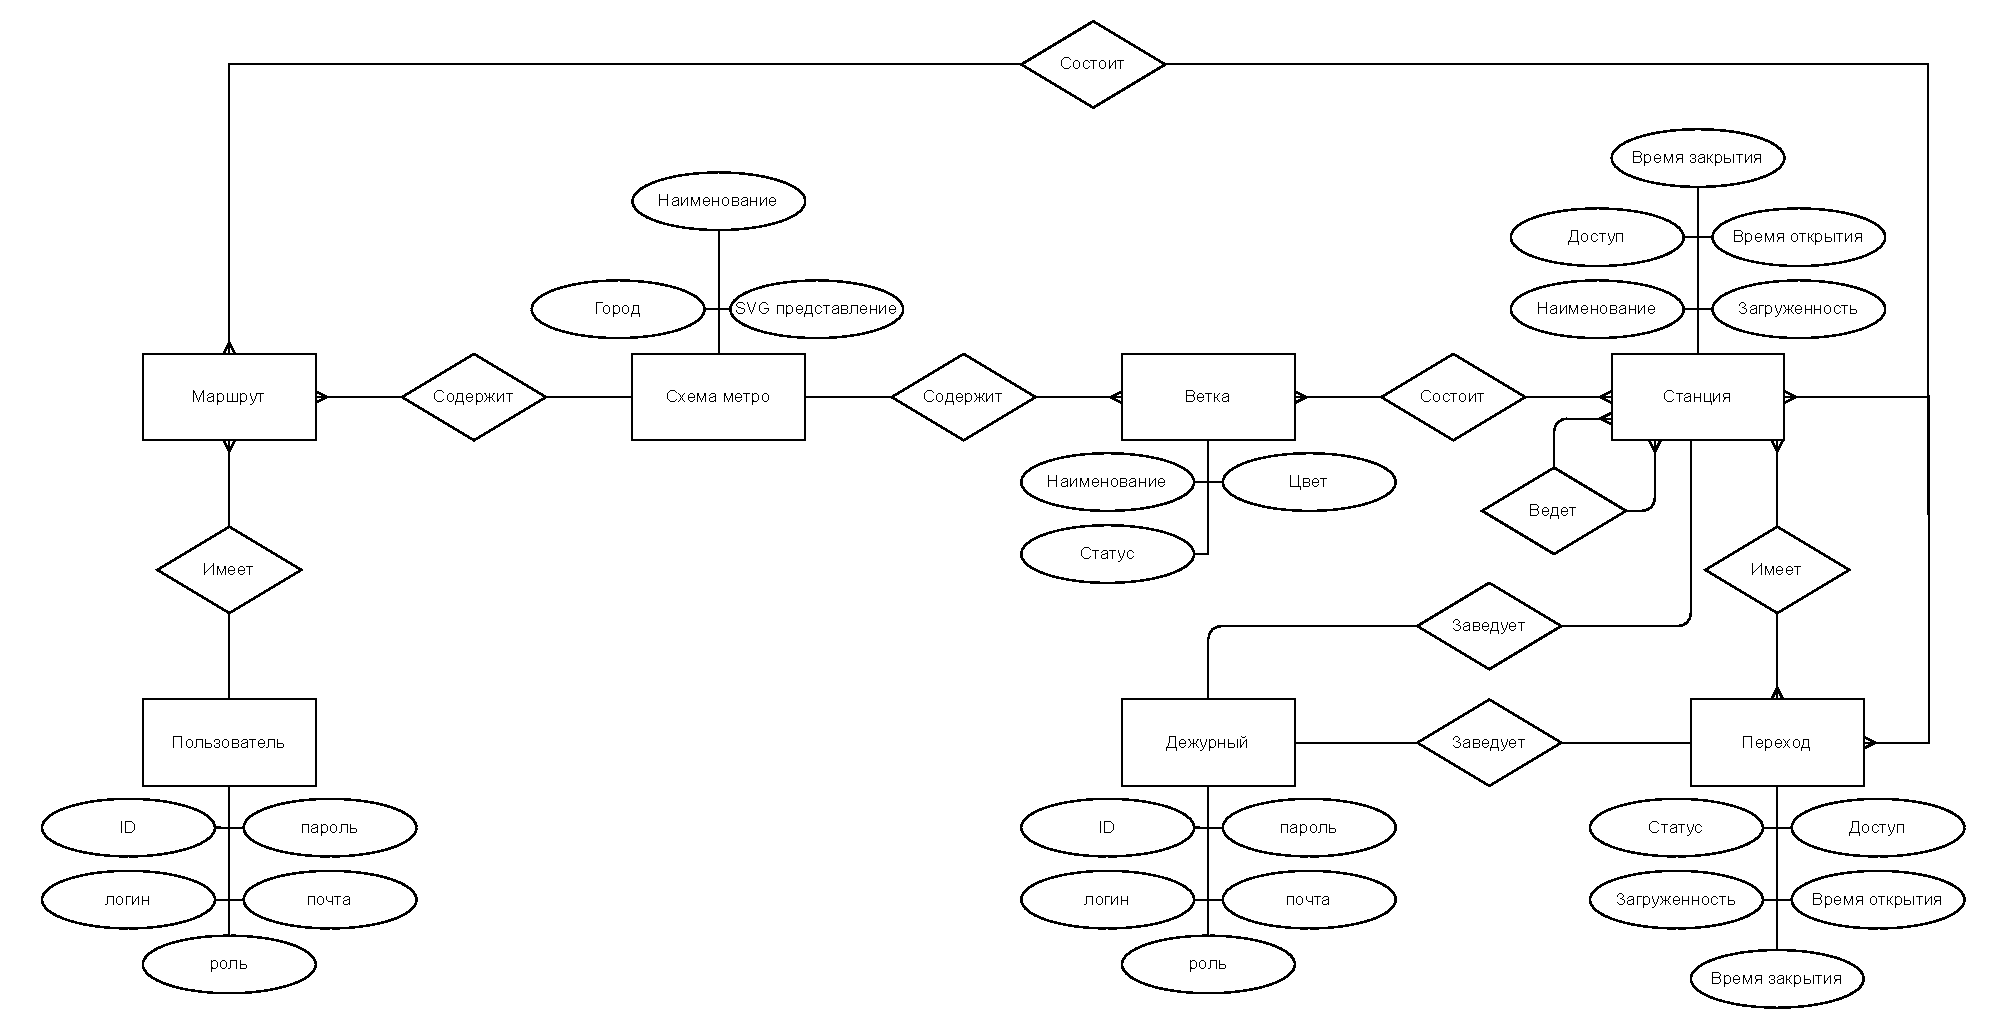
\includegraphics[width=\textwidth]{inc/img/ER.pdf}
    \caption{Диаграмма связей сущностей}
    \label{chart:er}
\end{figure}

\FloatBarrier
